\section{Kialakulás}
A relációs adatbázis kifejezés Edgar Frank Codd\footnote{Brit matematikus, informatikus, az IBM kutatójaként dolgozott} nevéhez fűződik, egy 1970-ben kiadott, a ,,A Relational Model of Data for Large Shared Data Banks'' című cikkében használta először a fogalmat, és írta le 12 pontban mit ért a kifejezés alatt. 

\section{Jellemzők}

A relációs adatbázis-kezelő szoftverek közül a vállalati szegmensben a legelterjedtebb az Oracle Database\nomenclature{Oracle Database}{\hfill\\Az Oracle Corporation egyik legismertebb terméke, relációs adatbázis-kezelő rendszer} és a Microsoft SQL Server\nomenclature{Microsoft SQL Server}{\hfill\\Microsoft relációs adatbázis-kezelő rendszere, nagy népszerűségnek örvend, mivel fizetős alkalmazásokban is ingyenesen használható (az Express verzió).}. (\cite{rdbms_stat})\\ A webes alkalmazásoknál előszeretettel alkalmazzák a MySQL\nomenclature{MySQL}{\hfill\\Az egyik legismertebb relációs adatbázis-kezelő rendszer, 2010 óta az Oracle Corpotation tulajdona, egyszerű a használata és könnyen integrálható a legtöbb programozási nyelvvel} és  a PostgreSQL\nomenclature{PostgreSQL}{\hfill\\Open-source relációs adatbázis-kezelő rendszer, a teljesen ingyenes használhatósága miatt közkedvelt mind az ingyenes, mind a fizetős alkalmazások között.} terméket, illetve a mobiltelefonokban az alacsony erőforrásigényéről ismert SQLite\nomenclature{SQLite}{\hfill\\Kisméretű relációs adatbázis-kezelő rendszer. Az SQLite adatbázisnak nincs szerverkomponense, az adatbázis mindössze egy fájlból áll. A kis mérete és kompaktsága miatt szívesen alkalmazzák mind okostelefonokon, mind asztali alkalmazásokban (böngészők).} adatbázist. Az előző felsorolásból kitűnik, hogy a relációs adatbázisok felhasználási lehetőségei igen széleskörűek, hiszen egy bonyolult ERP rendszer, és a mobiltelefonon futó email kliens is ugyanarra az adatbázisrendszerre épít.
A relációs adatbázisokban az információk táblákba rendeződnek, amelyeknek kötött formája van, mivel előre meg kell határozni milyen oszlopok fognak szerepelni, illetve az oszlopoknak meg kell adni az adattípusát (szöveg, egész szám, lebegőpontos szám, dátum, bináris adat, megjegyzés). Az adatok beviteléhez, és listázásához (legyen az akár egy grafikus felülettel ellátott adatbázis-kezelő alkalmazás) az SQL\nomenclature{SQL (Structured Query Language)}{\hfill\\Általában a relációs adatbázis-kezelők által használt lekérdező nyelv.\\Megalkotása az 1970-es években történt az IBM-nél.} lekérdező nyelv használható, mellyel relációs műveletek segítségével kapható meg a megfelelő információ.

\subsection{Előnyök}

\begin{description}
	\item[Relációk] \hfill \\
		Mivel a legtöbb adat felírható valamilyen relációs formában vagy legalább összekapcsolható egy relációs művelettel, ezért az adatbázisban szereplő rekordok kapcsolatban vannak egymással.
	\item[Konzisztencia] \hfill \\
		A táblák egymás közötti hivatkozásait és idegen kulcsait az adatbázis ellenőrzi, amelyből következően megakadályozza a rossz hivatkozások létrejöttét.\\
		Például egy könyvtári rendszer adatbázisában, olyan könyv nem törölhető, melyre van hivatkozás a jelenleg kint lévő könyveket tartalmazó táblában.
	\item[Indexelés] \hfill \\
		Az adatbázisban történő keresést az indexelés jelentősen felgyorsítja, mivel az index fájlban eltárolásra kerülnek az indexelt oszlopban található adatra történő hivatkozások, és a keresés az index fájlban történik.
	\item[Redundancia megszüntetése] \hfill \\
		Minden relációs rendszer a redundanciamentességre, azaz az adatok többszöri jelenlétének elkerülésére törekszik.
	\item[Tranzakciók] \hfill \\
		A tranzakciók segítségével egy komplex adatbeillesztés (több lépésből álló adatbeszúrások) hibája esetén, felmerülő félig beillesztett rekordok elkerülhetőek, ugyanis hiba esetén a tranzakció visszavonható. \\
		A tranzakciók a pénzügyi rendszerek egyik alapjai.

\end{description}

\subsection{Hátrányok}
	\label{subsect:reldbdisa}
\begin{description}
	\item[Rugalmatlanság] \hfill \\
		Egy relációs adatbázis kevésbé flexibilis, mert nehezen követi az inkrementális fejlesztés változó követelményeit, problémákat okozhat a verziókövetés, a visszafelé kompatibilitás. További problémák lehetnek például:
		\begin{itemize}
			\item a különböző tulajdonságokkal rendelkező entitások leírása: \\
			például egy címjegyzék, ahol a kapcsolatok nagy részének egy vagy kettő telefonszáma van, de előfordulhat a három telefonszám, email cím, beosztás és még az egyes kontaktokhoz létrehozott egyéni mezők kombinációja is.
			\item a hézagos adatfeltöltések: például az adóbevallás, ahol mindenkinél szerepel minden kitölthető mező, viszont a kitöltők mindössze a mezők töredék részét töltik ki.
		\end{itemize}
	\item[Relációk] \hfill \\
		A legtöbb információ leírható relációkkal, azonban egy közösségi oldalnál, ahol a felhasználók rengeteg mezőt kitölthetnek (név, lakcím, iskolák, email címek, stb.), és még saját mezőket is felvehetnek, gyakran a relációs megközelítés szuboptimális, a nagy adathalmazon mérhető keresési idők miatt. A problémát jól szemléltetheti egy gyógyszeradatbázis, ahol ki kell tölteni minden gyógyszer alapanyagát, amely viszont sok oszlopot eredményez a táblákban - hézagos kitöltés és \emph{NULL} értékek megadása a relációkat felboríthatja.\\
		Gyakran a sok relációval leírt adatok lekérdezése időigényes lehet, illetve sok információt nehéz leírni relációval, vagy az adatbázist feleslegesen bonyolulttá teszi. Megfigyelhető, hogy a komolyabb adattárházakban nem minden adatbázis a lehető legoptimálisabb, mivel dönteni kell a teljesítmény és az áttekinthetőség között.
	\item[Fregmentáció] \hfill \\
		Az adatbázis bináris fájlként kerül tárolásra a lemezen. Ha az adatbázis séma módosul egy új oszlop hozzáadásával, azt az adatbázis-kezelő rendszer már nem tudja  a lemezen a korábban felvett oszlopok mellé menteni, hanem a következő szabad részre kerül, így az adott táblából történő olvasáskor a diszk olvasófeje folyamatosan ugrálni fog, a válaszidők meghosszabbodását okozva. Hasonlóan problémát jelenthet egy oszlop törlése, mivel az adatbázis fizikai méretének csökkenésével nem jár. Az adatbázis fájlszerkezetét leginkább a FAT\nomenclature{FAT fájlrendszer}{\hfill\\Eredetileg az MS-DOS fájlrendszere, később a Microsoft Windows is ezt használta. Az adattárolás során a nagy szektor méretek miatt, a fájlrendszer pazarlóan bánt merevlemezen tárolókapacitásával.} fájlrendszerhez lehetne hasonlítani, ahol a fregmentáció miatt gyakran szükséges töredezettségmentesítést futtatni.\\
		Ez a probléma nem érinti az adatbázisban tárolt megjegyzéseket és bináris állományokat, mert azok az adatbázisrendszer külön tárolja (az oszlop méret flexibilis mivolta miatt).
	\item[Hosszú válaszidők] \hfill \\
		A nagy adatbázisoknál gyakori probléma, hogy a sok relációs kapcsolat hosszú válaszidőket okoz (soktáblás JOIN műveletek).
	\item[Bináris fájltárolási problémák] \hfill \\
		A legtöbb relációs adatbázis támogatja a fájlok tárolását, azonban egy-egy fájllekérés hatalmas plusz terhelést ad a szervernek, így általában a gyakorlatban nem alkalmazzák.
	\item[Memória (optimális) kihasználása] \hfill \\
		Az egyes adatbázisrendszerek nem, vagy nem optimálisan használják ki a memória által nyújtott cachelési lehetőségeket. Ennek egyik oka, hogy a 32 bites architektúrákban a memória maximum 3 gigabájtig címezhető, így az adatbázis-kezelő mindig a lemezre írja, és a lemezről olvassa az információkat, hosszú válaszidőket eredményezve.
\end{description}

%\chapter{SQL}
%Az SQL (Structured Query Language) nyelven keresztül férhetünk hozzá a relációs adatbázisunkban lévő információkhoz, ez a többi programozási nyelvtől eltérően eléggé beszélő (régebben SEQUEL\nomenclature{SEQUEL (Structured English Query Language)}-nek is nevezték
\section{ORM\\\small{Object-relational mapping}}
\label{ORM}
Az ORM egy olyan programozási technika, melynek segítségével egy relációs adatbázist objektumokká lehet konvertálni.\\
\hfill \\
\textbf{Miért van erre szükség?}
A ma használt programozási nyelvek legnagyobb része objektumorientált, azaz az adatbázisból érkező lekérdezések eredményét a memóriában objektumok formájában kell felépíteni.\hfill\\
A nagy adatbázisoknál a nagy adathalmaz miatt komoly problémát okoz a relációk felépítése a táblák között. \Aref{fig:wpdbstruct_o} ábra ezt kívánja szemléltetni.

\begin{figure}[h]
	
	\begin{minipage}{\textwidth}
		\begin{center}
			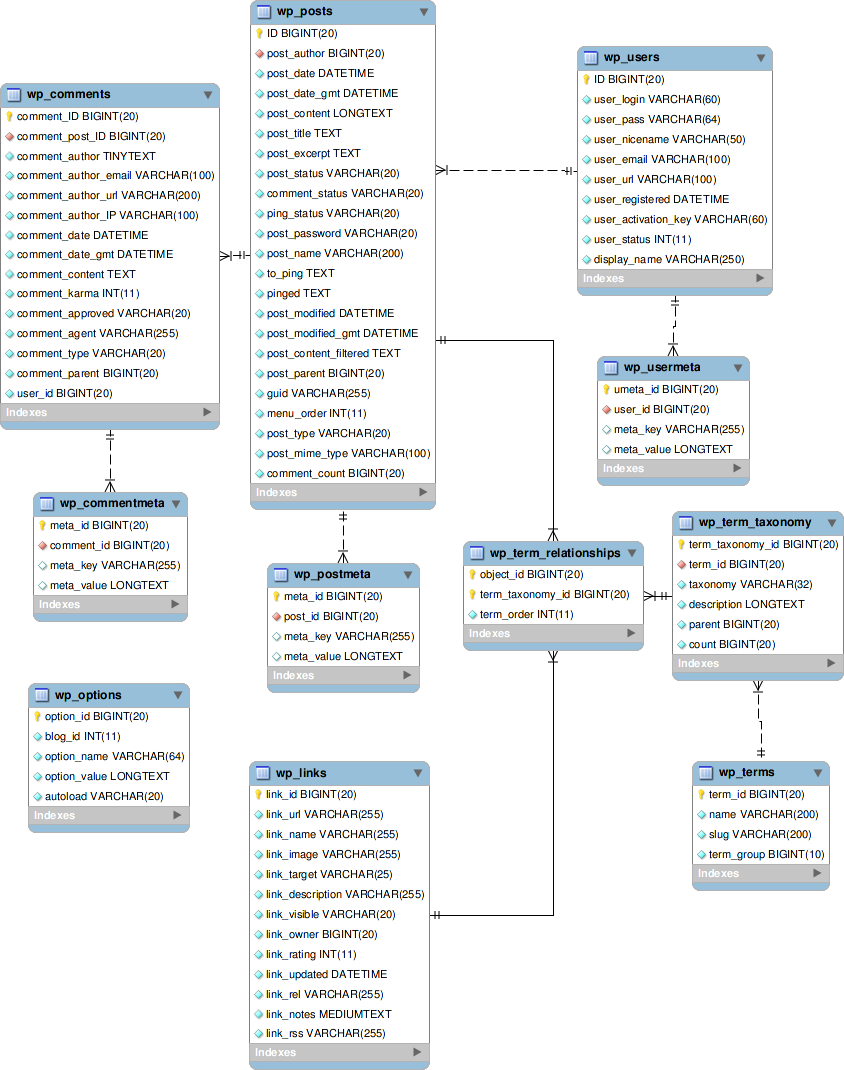
\includegraphics[scale=0.50]{pictures/wordpress_db_struct.png} %,height=80mm
		\end{center}
		\caption[DUMMY CAPTION]%
		{A népszerű Wordpress CMS\nomenclature{CMS (Content Management System)}{\hfill\\Tartalomkezelő rendszer, melynek segítségével programozói tudás nélkül lehetséges a weboldalak készítése} adatbázisának felépítése
		\hfill\\
A Wordpress, az egyik legismertebb PHP alapú tartalomkezelő rendszer. 2011. áprilisában közel 20 millió weboldalnál és blognál alkalmazták.\\
Az adatbázisának felépítése egyszerűnek mondható, bár itt is problémát okozhat a különböző táblák és a táblákban szereplő oszlopok fejben tartása. Egy ERP rendszernél, ahol több száz tábla is lehet, táblánként több tíz oszloppal az átláthatóság szinte lehetetlen.\\
		}
	\end{minipage}
\label{fig:wpdbstruct_o}
\end{figure}
\clearpage
\hfill\\
A ORM használatakor a programozási nyelv SQL mondatokká alakítja a kérést, majd az adatbázis által visszaadott választ a memóriában objektumokból felépülő listává alakítja, később az adatbázis írásakor az objektumokban történt változásokat visszaalakítja SQL mondatokká.\\
Fontos megemlíteni az ilyenkor használt két technikát, az optimista és a pesszimista zárolást.

\hfill\\\\
\textbf{Optimista zárolás}
Az optimista zárolás esetén a lekérdezés lefut, az adatok memóriába kerülnek, majd visszaíráskor dönti el az adatbázis időbélyegzők (timestamp) alapján, hogy frissült-e az adatbázis. Tehát míg az egyik kliens módosítja az információkat addig mások hozzáférhetnek az adatokhoz és akár ők is módosítják. Ez a megvalósítás akkor lehetséges, ha az alkalmazás használata közben feltételezhető, hogy két felhasználó egyszerre nem akarja módosítani az ugyanazt a rekordot, vagy nagyon kicsi az esélye az egyidejű adatmódosításnak.

\hfill\\\\
\textbf{Pesszimista zárolás}
A pesszimista zárolás esetén, ha egy kliens szerkesztésre megnyit az adatbázisban szereplő információkat, akkor az adott rekordok zárolásra kerülnek, majd a módosítás elküldése után válik lehetővé a többi kliens számára is a módosítás, tehát ha egy kliens szerkeszti az információkat, a többiek csak megtekinteni tudják azt, a módosítás nem lehetséges.\\
Ennél a megoldásánál problémát jelenthet a kliens leszakadása a hálózatról, ugyanis ilyenkor nem egyértelmű, hogy a zárolást mikor kell feloldani.\\
\hfill\\
Az, hogy optimista vagy pesszimista zárolást használjon egy alkalmazás, erősen függ a tárolt adatoktól. Például egy pénzügyi rendszer valószínűleg a pesszimista módszert fogja választani, míg egy egyszerű blognak megfelelő választás az optimista is.



